\documentclass[11pt,letterpaper]{article}
\usepackage[lmargin=1in,rmargin=1in,bmargin=1in,tmargin=1in]{geometry}
\usepackage{style/quiz}
\usepackage{style/commands}

% -------------------
% Content
% -------------------
\begin{document}
\thispagestyle{title}

% Quiz 1
\quizsol \textit{True/False}: The product $189.75(1.08)$ can be interpreted as representing finding either 8\% of $189.75$ or increasing $189.75$ by 8\%. \pspace

\sol The statement is \textit{false}. To compute a \% of some number $N$, we need only compute $N \cdot \%_d$ and if we want to compute $N$ increased or decreased by a \%, we compute $N \cdot (1 \pm \%_d)$, where $\%_d$ is the percentage written as a decimal and we choose `$+$' if it is an increase and choose `$-$' if it is a decrease. So thinking of the product $189.75(1.08)$ as finding a percent of a number, we must have $\#= 189.75$ and $\%_d= 1.08$, i.e. $\%= 108\%$. Then one way of interpreting this is finding 108\% of 189.75---not the 8\% claimed in the quiz statement. Interpreting the product $189.75(1.08)$ as finding a percentage increase/decrease, it must be a percentage increase because $1.08 > 1$. Writing $1.08= 1 + 0.08$, we can see that $\%_d= 0.08$. Therefore, $189.75(1.08)$ can represent finding 189.75 increased by 8\%---which is what is claimed in the quiz statement. \pvspace{1.3cm}



% Quiz 2
\quizsol \textit{True/False}: Suppose $R(x)$, $C(x)$, and $P(x)$ are revenue, cost, and profit functions. If $C(x) < R(x)$, then the company is making a profit and $P(x) > 0$. \pspace

\sol The statement is \textit{false}. If $C(x) < R(x)$, i.e. $R(x) > C(x)$, then the costs are less than the revenue; equivalently, the revenue is greater than the costs. But then the company should be making a profit, i.e. $P(x) > 0$. Alternatively, recalling that $P(x)= R(x) - C(x)$, if $R(x) > C(x)$, then $P(x)= R(x) - C(x) > 0$. But then the statement of the quiz is true. \pvspace{1.3cm}



% Quiz 3
\quizsol \textit{True/False}: If Prunella takes out a simple discount note with maturity \$5,000 for 3~months at 8.9\% annual interest, then she receives \$4,888.75 from the bank and pays a total of \$111.25 in interest. \pspace

\sol The statement is \textit{true}. We know that Prunella will receive the loan amount minus the interest. Observe that $\$4888.75 + \$111.25= \$5000$, which supports the claim in the quiz. We can verify this directly. The total interest paid on the loan, i.e. the discount, is $D= Mrt= \$5000(0.089) \frac{3}{12} \approx \$111.25$. Prunella then receives $\$5000 - \$111.25= \$4888.75$. Therefore, the statement of the quiz is true. At the end of the 3~months, Prunella owes the bank the full \$5,000 maturity of the loan---having paid the \$111.25 in interest up-front. In total, Prunella pays $\$5000 + \$111.25= \$5111.25$ for the loan. \pvspace{1.3cm}



% Quiz 4
\quizsol \textit{True/False}: If you invest \$9,000 at 3.3\% annual interest, compounded monthly, then the amount of money in the account after 2~years is given by $\$9000 \left(1 + \dfrac{0.33}{12} \right)^{12} \approx \$12,463.05$. \pspace

\sol The statement is \textit{false}. If one begins with a principal $P$ that earns an annual interest rate $r$, compounded $k$ times per year for $t$ years, then the final amount is $F= P \left(1 + \frac{r}{k} \right)^{kt}$. Here, the principal is $P= \$9000$, the annual interest rate is $r= 0.033$, $t= 2$~years, and $k= 12$ because the interest is compounded monthly. But then we have\dots
	\[
	F= P \left(1 + \frac{r}{k} \right)^{kt}= \$9000 \left(1 + \dfrac{0.033}{12} \right)^{12 \cdot 2}= \$9000 (1.00275)^{24}= \$9000 (1.06812996) \approx \$9,\!613.17
	\]
Therefore, the quiz statement is false. Observe they have $r= 0.33$ instead of $r= 0.033$. Furthermore, the exponent is the number of compounds per year, $k= 12$, rather than the total number of compounds $kt= 12 \cdot 2= 24$. \pvspace{1.1cm}



% Quiz 5
\quizsol \textit{True/False}: The greater the amount of money you place into an account earning 2.03\% yearly interest, compounded quarterly, the greater the effective interest. \pspace

\sol The statement is \textit{false}. We know the effective interest for an account with principal $P$ earning an annual interest rate $r$, compounded $k$ times per year is given by $\left(1 + \frac{r}{k} \right)^k - 1$. Observe that this does not depend on $P$. Therefore, the effective interest is independent of the amount of money in an account. This makes sense because the effective interest is an annual interest \textit{rate} and should be independent of account amounts. Of course, the greater the amount in the account, the greater the amount of interest earned; however, this does not affect the \textit{rate} at which this amount was earned---the effective interest. As an aside, in this case, the effective interest rate is\dots
	\[
	r_{\text{eff}}= \left(1 + \dfrac{r}{k} \right)^k - 1= \left(1 + \dfrac{0.0203}{4} \right)^4 - 1= 1.005075^4 - 1= 1.0204551 - 1= 0.0204551
	\] \pvspace{1cm}



% Quiz 6
\quizsol \textit{True/False}: You save for a new car by making deposits of \$500 at the start of every month into a savings account. The account earns 1.7\% annual interest. This is an example of a simple annuity-immediate. \pspace

\sol The statement is \textit{false}. The payments are made at the start of every month, i.e. at the start of every payment period. Therefore, this is an annuity due. The account earns interest annually but the deposits are made monthly. Therefore, this is a general annuity due. This shows the quiz statement is false. \pvspace{1.1cm}



% Quiz 7
\quizsol \textit{True/False}: If you had an amortized loan for \$150,000 at 9.4\% annual interest, compounded monthly with monthly payments over 30~years, then the minimum payments would have to be at least $\frac{\$150000}{12 \cdot 30}= \frac{\$150000}{360} \approx \$416.67$. \pspace

\sol The statement is \textit{true}. If one makes monthly payments over 30~years, a total of $12 \cdot 30= 360$ payments are made. If the loan had no interest and only the principal was expected to be repaid using 360~equal payments, then each payment would have to be $\frac{\$150000}{12 \cdot 30}= \frac{\$150000}{360} \approx \$416.67$. Clearly, the loan will have interest so that payments will have to be at least this amount; that is, \$416.67 is the absolute smallest amount the monthly payments could be to repay this loan. In fact, this bound is not very `sharp.' For instance, if the payments were at the end of each month, then the monthly payments would be\dots
	\[
	R= \dfrac{P}{a_{\actuarialangle{360\,}\, 0.00783333}}= \dfrac{\$150000}{119.966236} \approx \$1,\!250.35
	\]



\newpage



% Quiz 8
\quizsol \textit{True/False}: If $A, B$ are independent events with nonzero probability, then $P(A \text{ and } B)= P(A) \cdot P(B)$, $P(A)= P(A \;|\; B)$, and $P(B)= P(B \;|\; A)$. \pspace

\sol The statement is \textit{true}. Two events $A, B$ are called independent if and only if $P(A \text{ and } B)= P(A) \cdot P(B)$. Therefore, the first statement of the quiz must be true. If $A$ and $B$ are independent, then the occurrence or non-occurrence of $A$ does not affect the probability of $B$ and vice versa. We know that $P(A \;|\; B)$ is the probability of $A$ given that $B$ occurs. But if $A, B$ are independent, then $B$'s occurrence does not change the probability that $A$ occurs. But then $P(A \;|\; B)= P(A)$. Similarly, $P(B \;|\; A)= P(B)$. We can see this directly from the definition of $A$ and $B$ being independent: $P(A \text{ and } B)= P(A) \cdot P(B)$. If this is true, then\dots
	\[
	P(A \;|\; B)= \dfrac{P(A \text{ and } B)}{P(B)}= \dfrac{P(A) P(B)}{P(B)}= P(A), \qquad P(B \;|\; A)= \dfrac{P(B \text{ and } A)}{P(A)}= \dfrac{P(B) P(A)}{P(A)}= P(B)
	\] \pvspace{1.3cm}



% Quiz 9
\quizsol \textit{True/False}: You survey 150 people about their movie likes/dislikes and 58 say they like horror, 73 say they like comedy, with 13 saying they like both, then the probability that a randomly selected person likes horror or comedy is $\frac{58 + 73 + 13}{150}= \frac{144}{150} \approx 0.96$. \pspace

\sol The statement is \textit{false}. If one finds the number of people that enjoy horror or comedy by adding $58 + 73 + 13= 144$, then one has counted the 13~people that like horror and comedy once in the 58~people that enjoy horror and then again when one includes the 73~people that enjoy comedy. To avoid overcounting, one need \textit{subtract} the 13~people that enjoy both. So the probability that a randomly selected person likes horror or comedy is $\frac{58 + 73 - 13}{150}= \frac{116}{150} \approx 0.7733$. Alternatively, one can apply the rules of probability:
	\[
	P(\text{horror or comedy})= P(\text{horror}) + P(\text{comedy}) - P(\text{horror and comedy})= \dfrac{58}{150} + \dfrac{73}{150} - \dfrac{13}{150}= \frac{116}{150} \approx 0.7733
	\] \pvspace{1.3cm}



% Quiz 10
\quizsol \textit{True/False}: If $S= \{ s_1, s_2, \ldots, s_n \}$ is a finite sample space and $f$ is a random variable on $S$, then the expected value of $f$ is simply the average value of the numbers $f(s_1), f(s_2), \ldots, f(s_n)$. \pspace

\sol The statement is \textit{false}. For example, consider flipping a biased coin with probability $\frac{99}{100}$ of heads and $\frac{1}{100}$ of tails. Suppose you win \$100 if flip tails and \$0 if you flip heads. That is, we have $S= \{ \text{H}, \text{T} \}$ and the random variable $f(\text{H})= 0$ and $f(\text{T})= 100$. Clearly, `the majority' of the time you win nothing. On average, every 100 flips you win \$100. So we expect an average winning of \$1. But if we average these two outputs, we obtain $\frac{\$0 + \$100}{2}= \frac{\$100}{2}= \$50$. Recall that the expected value, or mean, of a discrete random variable is $\sum f(X) P(x= X)$; that is, we weight the value by the probability of seeing that value. The example above shows that these need not always align. \pvspace{1.3cm}



% Quiz 11
\quizsol \textit{True/False}: Suppose you are playing a game with finite sample space $S$. The payouts for events in the sample space are given by a random variable, $X$. If the expected value of $X$ is positive, i.e. E$X > 0$, then you always make money playing this game. \pspace

\sol The statement is \textit{false}. Suppose you win \$1,000,000 if you flip a heads on a fair coin and lose \$1 if you flip a tails. You flip the coin once and obtain tails. You have just lost money despite the fact that the expected value is\dots
	\[
	EX= \sum f(X) P(x= X)= \$1,\!000,\!000 \cdot \dfrac{1}{2} + (-\$1) \cdot \dfrac{1}{2}= \$499,\!999.50
	\]
The expected value only says what occurs \textit{on average in the `long run.'} So what we do expect is that having flipped the coin `sufficient' times, say 1,000 or 10,000 or millions, etc., of times that the average amount won/lost per would be \$499,999.50. One can then estimate the expected amount won/lost by computing \$499,999.50$n$, where $n$ is the number of games. So E$X > 0$ only means that one expects the average amount won per game in the long run to be positive. The expected value does not make a explicit prediction about what happens in a particular sequence of trials. \pvspace{1.3cm}



% Quiz 12
\quizsol \textit{True/False}: Let $x, y$ be random samples drawn from a normal distribution. If $z_x= -3.87$ and $z_y= 1.15$, then $y > x$ but $x$ is the more `unusual' value. \pspace

\sol The statement is \textit{true}. Recall that $z_x= \frac{x - \mu}{\sigma}$. The difference $x - \mu$ tells you the distance from $x$ to $\mu$. Thus, $\frac{x - \mu}{\sigma}$ tells you the number of standard deviations $x$ is from $\mu$. If $z_x < 0$, then $x < \mu$; if $z_x= 0$, then $x= \mu$; if $z_x > 0$, then $x > \mu$. For a normal distribution, we know the further $x$ is from the mean, the more `unusual' the value is, i.e. the less probable values at least extreme as $x$ are. Now because $|z_x|= 3.87 > 1.15= |z_y|$, $x$ is more standard deviations from $\mu$ than $y$, i.e. $x$ is more `unusual' than $y$. Because $z_x < 0$ and $z_y> 0$, $x$ is less than $\mu$ and $y$ is greater than $\mu$. \pvspace{1.3cm}



% Quiz 13
\quizsol \textit{True/False}: You take a random sample of 1,000 Democrats about whether they support Congress's immigration policies. The count of those that do not support Congress's immigration policies will be given by a binomial distribution. \pspace

\sol The statement is \textit{false}. To be a binomial distribution, a count $X$ must satisfy the following: (i) there are a fixed number of trials $n$, (ii) the event either occurs or does not with each observation, (iii) the probability of observing the event is independent, and (iv) the observations must be independent. In this instance, we have a fixed number of trials---1,000. If the survey has a binary response---support or not---then the event either occurs or does not. However, the probability of observing a Democrat that supports Congress is likely not constant across Democrats. Moreover, because Democrats likely share similar opinions, the observations are not likely independent from each other. Therefore, the number of Democrats that support/do not support Congress from this sample of 1,000 individuals does not likely follow a binomial distribution. \pvspace{1.3cm}



% Quiz 14
\quizsol \textit{True/False}: Consider a binomial distribution $B(n, p)$. The larger the value of $n$, the more the binomial distribution ``looks like'' the normal distribution $N\big(np, \sqrt{np(1 - p)}\, \big)$. \pspace

\sol The statement is \textit{true}. Recall that a binomial distribution for counts, $X$, $B(n, p)$ has mean $\mu= np$ and standard deviation $\sigma= \sqrt{np(1 - p)}$. However, probabilities $P(X= k)$ need not be given by a normal distribution. However, it follows that when one takes a simple random sample from a `sufficiently large' population (approximately, one for which $np \geq 10$ and $n(1 - p) \geq 10$), then $B(n, p) \approx N(\mu, \sigma)$ with the same mean and standard deviation as the underlying binomial distribution. But then $B(n, p) \approx N\big(np, \sqrt{np(1 - p)}\, \big)$. \pvspace{1.3cm}



% Quiz 15
\quizsol \textit{True/False}: The margin of error for a confidence interval is $z^* \frac{\sigma}{\sqrt{n}}$ and the larger the sample size, the smaller the margin of error. \pspace

\sol The statement is \textit{true}. From the Central Limit Theorem, if one takes a simple random sample $n$ from a population with mean $\mu$ and standard deviation $\sigma$ of `sufficiently large size' (approximately, $n \geq 30$), then a confidence interval with confidence $C$ is an interval of the form $\overline{x} \pm z^* \frac{\sigma}{\sqrt{n}}$, where $z^*$ is the number of standard deviations required so that $C$ percent of values are located $z^*$ standard deviations from $\mu$ in $N(1, 0)$. The margin of error is $\text{M.O.E.}= z^* \frac{\sigma}{\sqrt{n}}$---the maximum distance a value in the confidence interval is from the estimate $\overline{x}$. Observe that the large the sample size, $n$, the larger $\sqrt{n}$. But then $\frac{1}{\sqrt{n}}$ is smaller so that $\frac{1}{\sqrt{n}} \cdot z^* \sigma= z^* \, \frac{\sigma}{\sqrt{n}}$ is smaller, i.e. the margin of error is smaller. \pvspace{1.3cm}



% Quiz 16
\quizsol \textit{True/False}: Let $\mathbf{u}= \langle 0, -1, 5, 4 \rangle$ and $\mathbf{v}= \langle 1, 9, 2, -3 \rangle$. Then $\mathbf{u} \cdot \mathbf{v}= \langle 0, -9, 10, -12 \rangle$. \pspace

\sol The statement is \textit{false}. There is no multiplication for vectors. The dot product of two vectors produces a scalar, i.e. a real number. We know that $\mathbf{u} \cdot \mathbf{v}= \sum_i u_i v_i$; that is, the dot product of two vectors is the sum of the product of the components. Therefore, we have\dots
	\[
	\mathbf{u} \cdot \mathbf{v}= \langle 0, -1, 5, 4 \rangle \cdot \langle 1, 9, 2, -3 \rangle= 0(1) + (-1)9 + 5(2) + 4(-3)= 0 - 9 + 10 - 12= -11
	\] \pvspace{1.3cm}



% Quiz 17
\quizsol \textit{True/False}: There is no linear system of equations with exactly 2,023 solutions. \pspace

\sol The statement is \textit{true}. A linear system of equations either has no solutions, one solution, or infinitely many solutions. But then there can be no linear system of equations with exactly 2,023 solutions. \pvspace{1.3cm}



% Quiz 18
\quizsol \textit{True/False}: If matrix below is the RREF of an augmented matrix coming from a system of equations, then the original system of equations had only one solution: $(x, y)= (2, -3)$.
	\[
	\begin{pmatrix}
	1 & 0 & 2 \\
	0 & 1 & -3 \\
	0 & 0 & 0 
	\end{pmatrix}
	\] \pspace

\sol The statement is \textit{true}. There are three rows to the matrix so that the original system of equations had three equations. Each column of the matrix---except the last column---corresponds to a variable in the original system of equations. Therefore, the original system of equations has two variables: $x_1, x_2$. From the RREF, we see that $x_1= 2$ and $x_2= -3$. But then all the variables have a fixed value so that the original system of equations has a unique solution---namely $(x_1, x_2)= (2, -3)$. The bottom zero row of the RREF corresponds to the fact that the original system of three equations had a redundant equation---meaning that only two of the equations were necessary to arrive at the solution $(x_1, x_2)= (2, -3)$. \pvspace{1.3cm}



% Quiz 19
\quizsol \textit{True/False}: If one performs a linear regression and finds $r= 0.80$, then the variables are positively correlated and the coefficient of determination is $0.64$. \pspace

\sol The statement is \textit{true}. The (Pearson) correlation coefficient, $r$, determines whether the variables are positively or negatively correlated. If $r > 0$, the variables are positively correlated. If $r < 0$, the variables are negatively correlated. If $r= 0$, the variables are not correlated. Furthermore, the coefficient of determination, $r^2$, gives the `percentage' linearity; that is, $r^2$ gives the percentage of variability in the data explained by the model. We have $r^2= (0.80)^2= 0.64$. \pvspace{1.3cm}



% Quiz 20
\quizsol \textit{True/False}: Any linear function on a nonempty, bounded region has a maximum and a minimum value and these values are obtained at a corner point for the region. \pspace

\sol The statement is \textit{true}. This is the Fundamental Theorem of Linear Programming. For instance, the function $z= -2x_! + 5x_2$ on the region given by $-x_1 + x_2 \leq 4$, $4x_1 + x_2 \leq 24$, and $x_1, x_2 \geq 0$ meets these criterion: $z$ is a linear function in $x_1, x_2$, the region (shown below) is bounded, and the region is nonempty. 
	\[
	\fbox{
	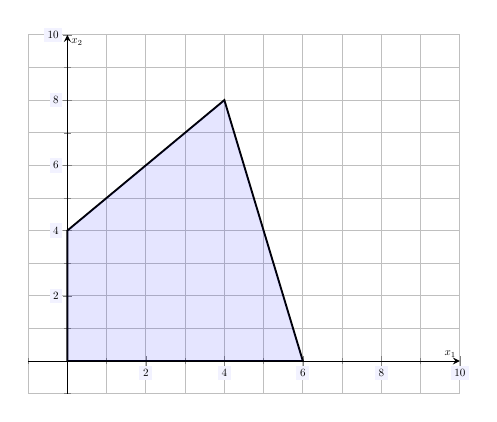
\begin{tikzpicture}[scale=0.8,every node/.style={scale=0.5}]
	\begin{axis}[
	grid=both,
	axis lines=middle,
	ticklabel style={fill=blue!5!white},
	xmin= -1, xmax=10,
	ymin= -1, ymax=10,
	xtick={0,2,4,6,8,10},
	ytick={0,2,4,6,8,10},
	minor tick = {-1,0,1,...,10},
	xlabel=\(x_1\),ylabel=\(x_2\),
	]
	\draw[line width=0.03cm] (0,0) -- (0,4) -- (4,8) -- (6,0) -- (0,0);
	\draw[line width=0.01cm,fill= blue,opacity=0.1] (0,0) -- (0,4) -- (4,8) -- (6,0) -- (0,0);
	\end{axis}
	\end{tikzpicture}
	}
	\]
Therefore, we only need evaluate the function on the corner points. 
	\begin{table}[!ht]
	\centering
	\begin{tabular}{l|l}
	$(x, y)$ & $z= -2x + 5y$ \\ \hline
	$(0, 0)$ & $z= 0 + 0= 0$ \\
	$(0, 4)$ & $z= 0 + 20= 20$ \\
	$(4, 8)$ & $z= -8 + 40= 32$ \\
	$(6, 0)$ & $z= -12 + 0= -12$
	\end{tabular}
	\end{table} \par	
Therefore, the minimum value for $z$ is $-12$ and occurs at $(x_1, x_2)= (6, 0)$, and the maximum value for $z$ is $32$ and occurs at $(x_1, x_2)= (4, 8)$. However, a linear function on a nonempty, \textit{unbounded} region may or may not have a maximum or a minimum value. 













\end{document}